\chapter{Digital Twin Implementation}\label{ch:implementation}

As introduced in Section~\ref{sec:dt_design}, the \acrshort{dt} developed for this thesis was implemented from scratch, as no physical twin exists yet. As such, the hypothetical home described in Chapter~\ref{ch:hypothetical_home} was used as a starting point to develop the \acrshort{dt}.

The \acrshort{dt} is implemented as a \acrfull{rest} \acrfull{api}, which provides endpoints to read routines and data of appliances in the home, show the energy consumption of appliances during the day, and simulate the addition of new routines evaluating eventual conflicts with the existing routines. Using a \acrshort{rest} \acrshort{api} allows to separate the \acrshort{dt} functionalities from the presentation layer ensures that the \acrshort{dt} can be used by different clients, such as web applications, mobile applications, and other services. To showcase the uses of the \acrshort{dt} a frontend web application was also developed in this thesis.

To simplify development, a few assumptions and limitations were introduced, whose overcoming is left as a future development. First, the digital twin operates using only the 24 hours of the day, from 00:00 to 23:59. Taking this into account, the routines that the \acrshort{dt} evaluates are assumed to be repeated every day, in the same conditions. Second, the digital twin evalutates the state of appliances throughout the day only using the routines, and is not capable of detecting the manual activation of appliances. Third, the routines and appliances in the home are provided to the \acrshort{dt} as static files, which are not updated through time to reflect the status of the physical twin. These last two limitatons were necessary due to the fact that the \acrshort{dt} is developed from scratch, and no physical twin exists yet.

\section{REST API}

An \acrshort{api} is a set of definitions and protocols for building and integrating application software. It's sometimes referred to as a contract between an information provider and an information user—establishing the content required from the client (the request) and the content required by the server (the response)~\parencite{redhatinc.WhatRESTAPI2020}.

First introduced by Roy Fielding in his doctoral dissertation~\parencite{fieldingArchitecturalStylesDesign2000}, \acrshort{rest} is an architectural style for distributed hypermedia systems based on the HTTP protocol, which allows to build scalable web services. The paradigm is based on the concept of resources, which are identified by unique URIs, and can be manipulated using a set of predefined operations~\parencite{framlingProductAgentsHandling2003}.

In order for an \acrshort{api} to be considered \acrshort{rest}ful, it has to conform to these criteria~\parencite{redhatinc.WhatRESTAPI2020,fieldingArchitecturalStylesDesign2000}:
\begin{itemize}
    \item A client-server architecture made up of clients, servers, and resources, with requests managed through HTTP.
    \item Stateless communication, meaning no client information is stored between get requests and each request is separate and unconnected.
    \item Cacheable data that streamlines client-server interactions.
    \item A uniform interface between components so that information is transferred in a standard form, such as XML, JSON, or even plain text. This thesis uses JSON, which is one of the most common formats as it is lightweight and easy to read and write.
    \item A layered system that organizes each type of server (those responsible for security, load-balancing, etc.) involved the retrieval of requested information into hierarchies, invisible to the client.
    \item Code-on-demand (optional): the ability to send executable code from the server to the client when requested, extending client functionality. 
\end{itemize}

\subsection{Implementation}

The \acrshort{rest} \acrshort{api} is implemented in Python 3.11, using the FastAPI\footnote{\url{https://fastapi.tiangolo.com/}} library, which is a modern and high-speed web framework for building \acrshort{api}s. The FastAPI library was chosen for its simplicity and performance, as it is based on the Starlette\footnote{\url{https://www.starlette.io/}} framework, which is a lightweight \acrfull{asgi} toolkit for building high-performance services. Due to this, the \acrshort{dt} \acrshort{api} is capable of handling multiple requests concurrently, and is designed to be scalable and easy to maintain.

FastAPI also provides automatic generation of OpenAPI documentation, which is a standard for documenting \acrshort{rest} \acrshort{api}s. Figure~\ref{fig:backend_swagger} shows such documentation, which is displayed using the Swagger UI\footnote{\url{https://swagger.io/tools/swagger-ui/}}, a tool for visualizing and interacting with the \acrshort{rest} \acrshort{api} resources, based on the OpenAPI specification. The documentation provides a list of all the endpoints, the methods allowed for each endpoint, and the parameters that each endpoint accepts. The UI also provides examples of the possible responses for each endpoint, and detail information about the structure of the responses. Finally, the documentation provides a way to interact with the \acrshort{api} directly from the browser, by allowing to send requests to the endpoints and see the responses.

\begin{figure}
    \centering
    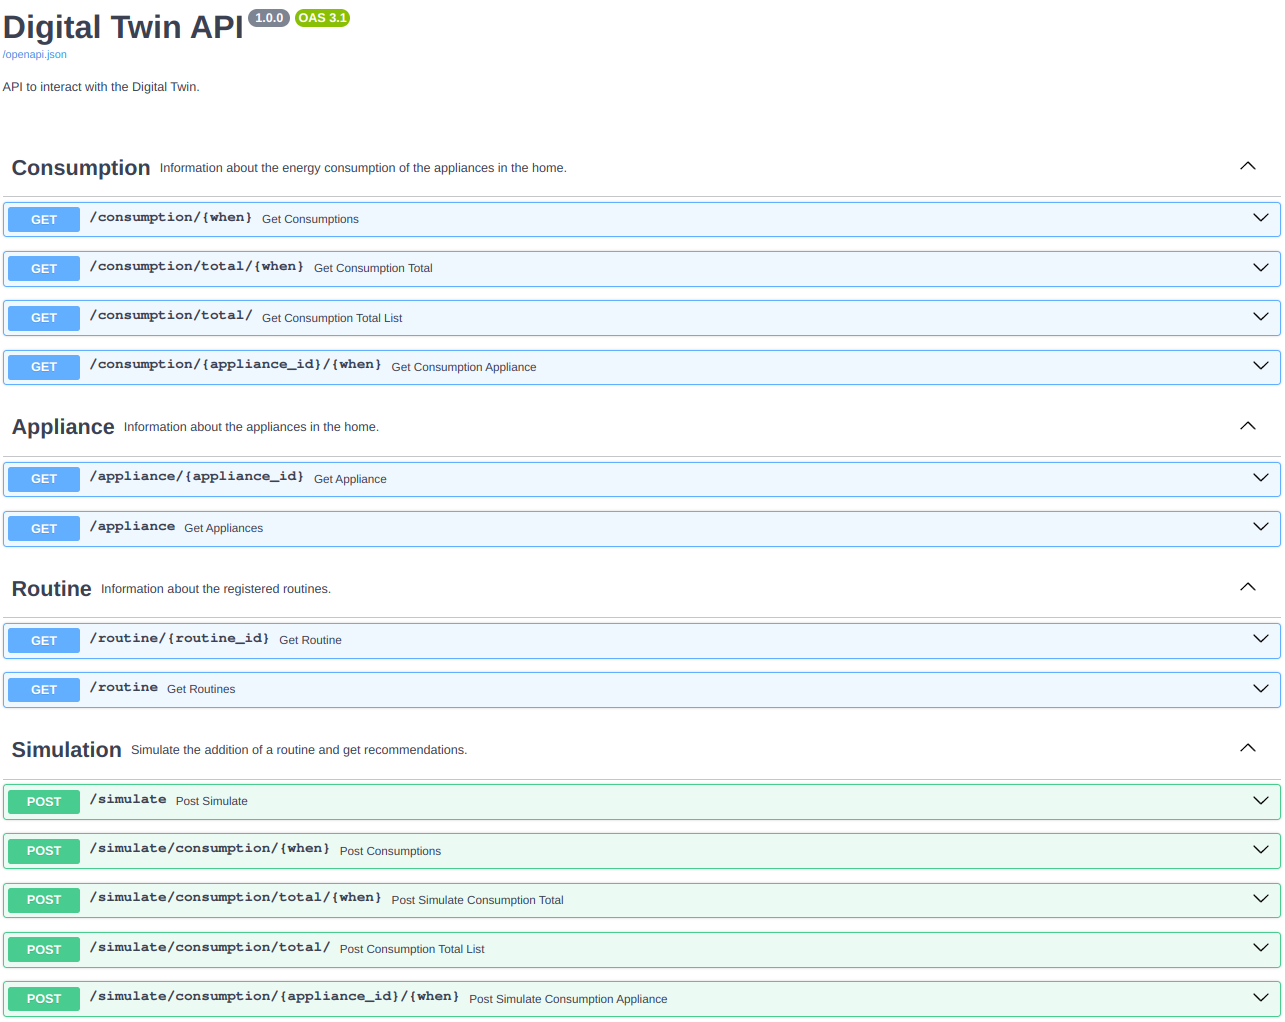
\includegraphics[width=\textwidth]{images/backend_swagger.png}
    \caption{Backend documentation generated by FastAPI}
    \label{fig:backend_swagger}
\end{figure}

Table~\ref{tab:rest_api_endpoints} shows all the endpoints of the \acrshort{dt}'s \acrshort{rest} \acrshort{api}. The \acrshort{dt} provides endpoints to read routines and data of appliances in the home, show the energy consumption of appliances during the day, and simulate the addition of new routines evaluating eventual conflicts with the existing routines. The \acrshort{dt} is capable of simulating the addition of a new routine, evaluating eventual conflicts with the existing routines, and providing recommendations and errors to the user. 

\begin{table}
    \centering
    \resizebox{\textwidth}{!}{%
        \begin{tblr}{ll>{\raggedright}p{.18\textwidth}p{.18\textwidth}lp{.5\textwidth}}
            \hline
            Endpoint                    & Method & Path parameters             & Query Parameters        & Body parameters     & Description                                                                                                                         \\ \hline
            /& GET    & &                         &                     & Displays the \acrshort{api} documentation using Swagger UI.                                           \\ \hline[dashed]
            /consumption                & GET    & date and time               &                         &                     & Returns a list of energy consumption values of all appliances at the given date and time.                                           \\
            /consumption                & GET    & appliance id, date and time &                         &                     & Returns the energy consumption value of the given appliance at the given date and time.                                             \\
            /consumption/total          & GET    &                             & list of dates and times &                     & Returns the list of total energy consumption of all appliances at the given dates and times.                                        \\
            /consumption/total          & GET    & date and time               &                         &                     & Returns the total energy consumption of all appliances at the given date and time.                                                  \\ \hline[dashed]
            /appliance                  & GET    &                             &                         &                     & Returns the list of all appliances                                                                                                  \\
            /appliance                  & GET    & appliance id                &                         &                     & Returns a specific appliance                                                                                                        \\ \hline[dashed]
            /routine                    & GET    &                             &                         &                     & Returns the list of all routines                                                                                                    \\
            /routine                    & GET    & routine id                  &                         &                     & Returns a specific routine                                                                                                          \\ \hline[dashed]
            /simulate                   & POST   &                             &                         & routine to simulate & Simulates the addition of a routine and returns a list of recommendations and errors (if any)                                       \\
            /simulate/consumption       & POST   & date and time               &                         & routine to simulate & Simulates the addition of a routine and returns a list of energy consumption values of all appliances at the given date and time    \\
            /simulate/consumption       & POST   & appliance id, date and time &                         & routine to simulate & Simulates the addition of a routine and returns the energy consumption value of the given appliance at the given date and time      \\
            /simulate/consumption/total & POST   & date and time               &                         & routine to simulate & Simulates the addition of a routine and returns the list of total energy consumption of all appliances at the given dates and times \\
            /simulate/consumption/total & POST   &                             & list of dates and times & routine to simulate & Simulates the addition of a routine and returns the total energy consumption of all appliances at the given date and time           \\ \hline
        \end{tblr}%
    }
    \caption{Endpoints of the \acrshort{dt}'s REST API}
    \label{tab:rest_api_endpoints}
\end{table}

\subsection{Example of Requests}

\begin{lstlisting}[language=plain,caption={Shape of the \acrshort{api} responses},label=code:api_response_shape,float,floatplacement=H]
{
    value[s]: ...
    error: {
        message: "...",
        context: {
            ...
        }
    }
}
\end{lstlisting}

The responses of the \acrshort{api} are standardized to the shape reported in Code Sample~\ref{code:api_response_shape}, which includes a \textit{value} field when the response is a single value, and a \textit{values} field when the response is a list of values. The response may also contain a \textit{error} field, which includes a \textit{message} field with a description of the error, and a \textit{context} field with additional information about the error.

\begin{lstlisting}[language=numbered,caption={Response to HTTP GET request to the \textit{/consumption/total} endpoint},label=code:api_response_consumption,float,floatplacement=H]
{
  value: 1578,
  error: null,
}
\end{lstlisting}

Submitting a \texttt{GET} request to the \texttt{/consumptions/total/2024-02-25T16:00} returns the total energy consumption of all appliances at 16:00 of the current day (the date part of the string is ignored) as shown in Code Sample~\ref{code:api_response_consumption}. The response contains a \texttt{value} field, with the total energy consumption in W, and the error field is \texttt{null}.

\begin{lstlisting}[language=numbered,caption={Response to HTTP POST request to the \texttt{/simulate} endpoint},label=code:api_response_simulate,float,floatplacement=H]
{
  values: [
    {
      "message": "Disable routine \"Wash Everything\"",
      "context": {
        "type": "DISABLE_ROUTINE",
        "routine_id": 3
      }
    },
    {
      "message": "Change start time of routine \"Party Time\"",
      "context": {
        "type": "CHANGE_START_TIME",
          "routine_id": 32,
          "when": "08:00"
      }
    }
  ],
  error: {
    "message": "Power consumption of the house is greater than 3.0kW at 09:59. This can cause a power cut-off.",
    "context": {
      "when": "09:59",
      "max_power": "3000"
    }
  }
}
\end{lstlisting}

Submitting a \texttt{POST} request to the \texttt{/simulate} endpoint with a routine in the body simulates the addition of such a routine, and returns a list of recommendations and errors. The response to a request containing a routine which brings the total consumption of the home over 3kW is shown in Code Sample~\ref{code:api_response_simulate}. The response contains a \texttt{values} field, with a list of recommendations, along with an \texttt{error} field. In this case, the response contains a recommendation to change the start time of the routine, another to disable a routine which causes high energy draw, and an error that the power consumption exceeds the maximum limit. The procedure for evaluating the conflicts and producing the recommendations and errors is described in detail in Section~\ref{sec:simulation}.

\section{Configuration}

\begin{lstlisting}[language=json,caption={Example of a configuration file.},label=code:configuration,float,floatplacement=H]
[energy]
max_power = 3
energy_rates_number = 2
energy_rates_prices = [
    0.131870,
    0.111492,
]

[database]
type = "json"
appliances_dir = "json/appliances"
routines_dir = "json/routines"
test_routines_dir = "json/test_routines"
\end{lstlisting}

The \acrshort{dt} supports a number of configuration parameters, set by a configuration file. The file must be written in TOML, and its location is set by the \texttt{CONFIG\_PATH} environment variable. The configuration file can contain the following information:
\begin{itemize}
    \item \texttt{energy}: energy related parameters.
          \begin{itemize}
              \item \texttt{max\_power}: the maximum power draw, in kW;
              \item \texttt{energy\_rates\_number}: the number of energy rates, e.g. 2 means dual-rate;
              \item \texttt{energy\_rates\_prices}: the price for each energy rate, in \texteuro/kWh.
          \end{itemize}
    \item \texttt{database}: database related parameters.
          \begin{itemize}
              \item \texttt{type}: the type of database, only \texttt{json} is supported at the moment;
              \item \texttt{appliances\_dir}: the directory where the appliances JSON files are stored;
              \item \texttt{routines\_dir}: the directory where the routine JSON files are stored;
              \item \texttt{test\_routines\_dir}: the directory where the routine JSON files for tests are stored;
          \end{itemize}
\end{itemize}

The number of energy rates supported by the \acrshort{dt} follows the Delibera n.181/06\footnote{\url{https://www.arera.it/atti-e-provvedimenti/dettaglio/06/181-06} (visited on 2024, February 22)} by the \acrfull{arera}, which defines the conditions for the application of multiple-rate tariffs. A maximum of three rates (F1, F2, F3) is allowed, where F1 goes from 8:00 to 19:00, monday to friday, F2 goes from 7:00 to 8:00 and from 19:00 to 23:00, monday to friday, and from 7:00 to 23:00 on saturday, and F3 goes from 23:00 to 7:00, monday to saturday, and from 23:00 to 24:00 on sunday. The allocation of the rates, represented in Figure~\ref{fig:costs_matrix} depends on the time of the day and the day of the week. The actual number of rates can be lower than three, depending on the contract with the energy provider. If only two rates are quoted, the rates F2 and F3 can be grouped to form a dual rate tariff (F1, F23).

\begin{figure}
    \centering
    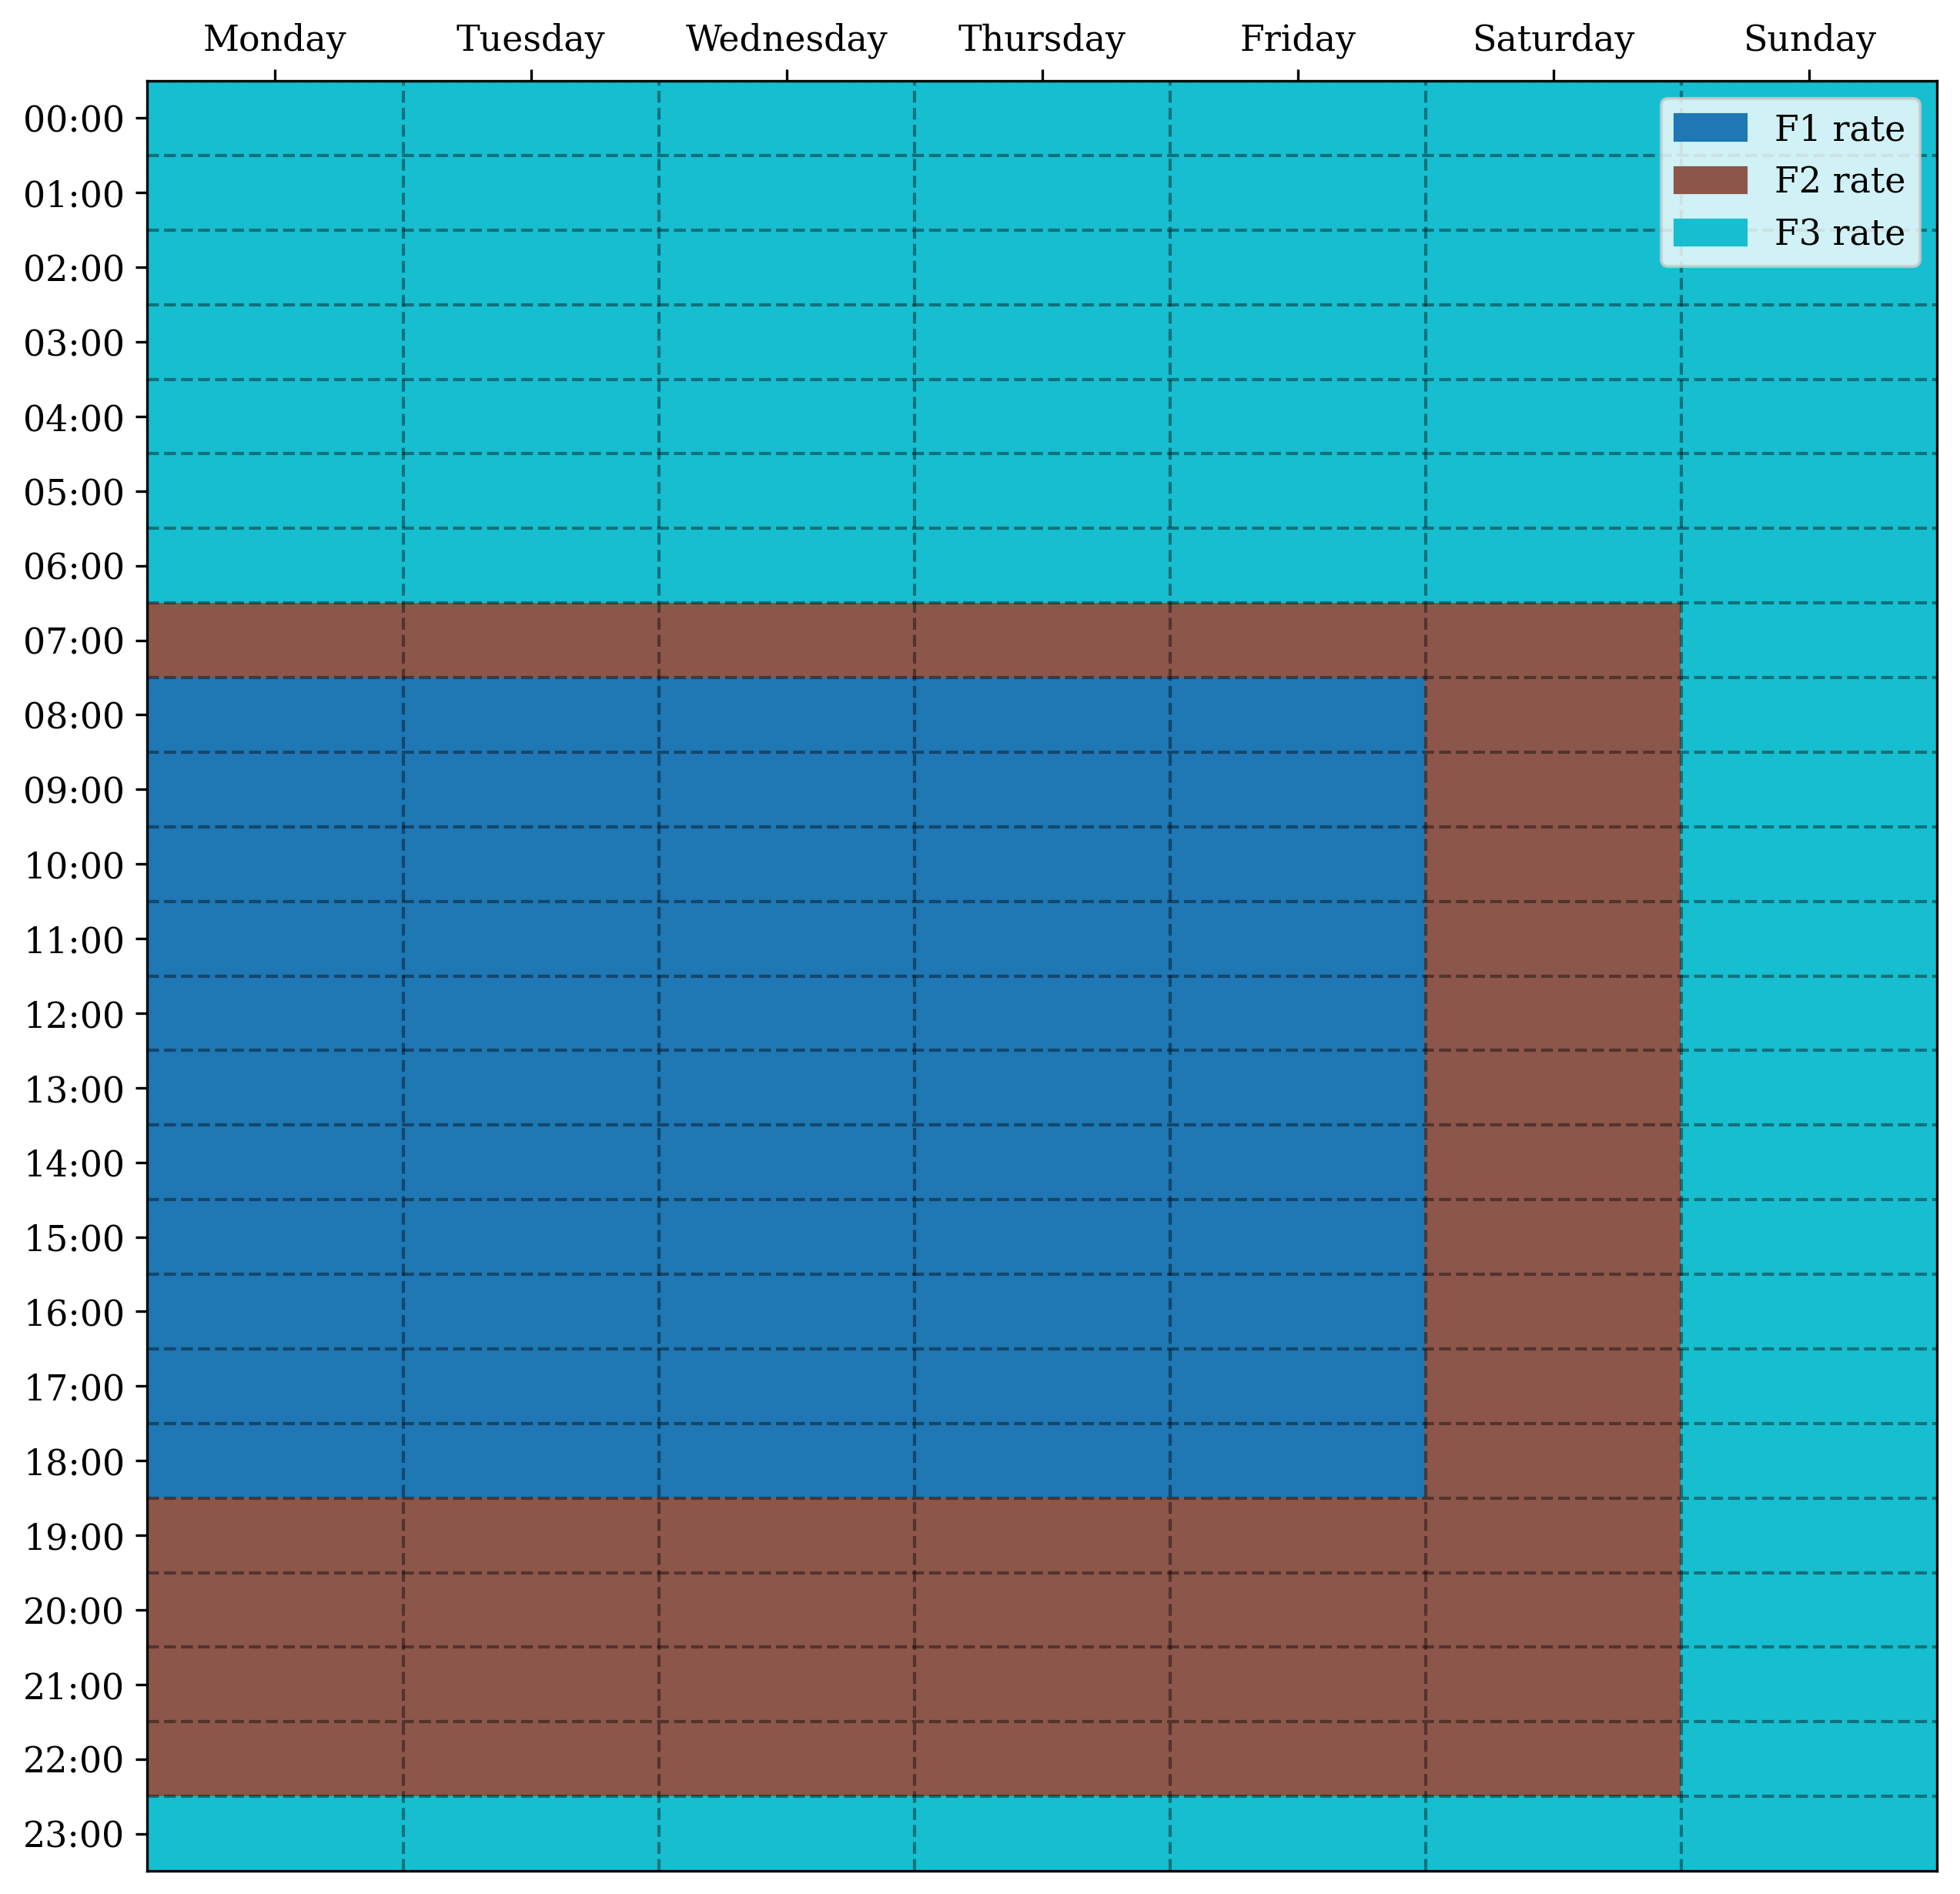
\includegraphics[width=0.9\textwidth]{images/costs.png}
    \caption[Electricity tariffs applied in italy for every day of the week]{Electricity tariffs applied in italy for every day of the week. F1 is the peak rate, F2 is the mid-level, and F3 is off-peak}
    \label{fig:costs_matrix}
\end{figure}

The configuration used for the development of the \acrshort{dt} is shown in Code Sample~\ref{code:config}. Two energy rates are used, where the prices correspond to the \acrfull{pun} values, i.e. the Single National Price values, refferring to the month of December 2023. The \acrshort{pun} is calculated by the \acrfull{gme}\footnote{\url{https://www.mercatoelettrico.org/En/default.aspx} (visited on 2024, February 22)}, as the weighted average of the prices of the energy markets, and is used as a reference for the energy costs in Italy. The maximum power draw is set to $3kW$, which is the standard maximum power supply before cut off in Italy.

\section{Appliance and Routine Data}

The data of the appliances in the hypothetical home and the routines registered by the end users are stored as JSON files.
Examples of appliance JSON files for the dish washer and the washing machine are shown in Code Samples~\ref{code:appliance_dish_washer} and~\ref{code:appliance_washing_machine}, respectively. The files contain the following information:
\begin{itemize}
    \item \texttt{id}: a unique integer number identifying the appliance among other appliances;
    \item \texttt{device}: the type of appliance, e.g. \textit{dish washer}
    \item \texttt{manufacturer} (optional): the manufacturer of the appliance, e.g. \textit{Whirlpool};
    \item \texttt{model} (optional): the model of the appliance e.g. \textit{ADF 555 IX};
    \item \texttt{location}: the room where the appliance is located, e.g. \textit{kitchen};
    \item \texttt{modes}: the list of operation modes available for the appliance. Every appliance has at least an \textit{off} mode, that consumes no power. For each mode the following information is provided:
          \begin{itemize}
              \item \texttt{id}: a unique integer number identifying the mode among the other modes of the appliance;
              \item \texttt{name}: the name of the mode, e.g. \textit{intensive};
              \item \texttt{power\_consumption}: the mean power consumption of the appliance in the mode, in Watts;
              \item \texttt{default\_duration} (optional): the default duration of the operation mode, which will be used if the user does not specify a duration in the routine.
          \end{itemize}
\end{itemize}

\begin{lstlisting}[language=numbered,caption={JSON file describing the dish washer},label=code:appliance_dish_washer,float,floatplacement=H]
{
  "id": 3,
  "device": "dish washer",
  "manufacturer": "Whirlpool",
  "model": "ADG 555 IX",
  "location": "kitchen",
  "modes": [
    {
      "id": 0,
      "name": "off",
      "power_consumption": 0
    },
    {
      "id": 1,
      "name": "daily",
      "power_consumption": 810,
      "default_duration": 10260
    },
    ...	
    {
      "id": 6,
      "name": "pre-wash",
      "power_consumption": 10,
      "default_duration": 660
    }
  ]
}
\end{lstlisting}

\begin{lstlisting}[language=numbered,caption={[JSON file describing the washing machine]JSON file describing the washing machine.},label=code:appliance_washing_machine,float,floatplacement=H]
{
	"id": 15,
	"device": "washing machine",
	"manufacturer": "Zanussi",
	"model": "F1215",
	"location": "bathroom",
	"modes": [
		{
			"id": 0,
			"name": "off",
			"power_consumption": 0
		},
		{
			"id": 1,
			"name": "cotton 90",
			"power_consumption": 2000,
			"default_duration": 8700
		},
		...	
		{
			"id": 7,
			"name": "wool",
			"power_consumption": 450,
			"default_duration": 3300
		}
	]
}
\end{lstlisting}

An example of a routine which starts the dish washer in \textit{intensive} mode and the washing machine in \textit{cotton 90} mode at 14:00 is shown in Code Sample~\ref{code:routine_wash_everything}. It should be noted that, as the routine file does not specify a duration for the operation modes set by the actions, the default duration modes of the respective actions will be used. The routine file contains the following information:
\begin{itemize}
    \item \texttt{id}: a unique integer number identifying the routine among other routines;
    \item \texttt{name}: a name for the routine, e.g. \textit{wash everything};
    \item \texttt{when}: the time when the routine is executed, in the format \textit{HH:MM};
    \item \texttt{actions}: the list of actions that the routine involves. For each action the following information is provided:
          \begin{itemize}
              \item \texttt{id}: a unique integer number identifying the action among the other actions of the routine;
              \item \texttt{appliance\_id}: the ID of the appliance involved in the action;
              \item \texttt{duration} (optional): the duration of the operation mode, in minutes. If not specified, the default duration of the mode is used.
          \end{itemize}
\end{itemize}

\begin{lstlisting}[language=numbered,caption={[Example of a routine with two actions]Example of a routine with two actions.},label=code:routine_wash_everything,float,floatplacement=H]
{
    "id": 5,
    "name": "Wash everything",
    "when": "14:00",
    "enabled": true,
    "actions": [
        {
            "id": 0,
            "appliance_id": 15,
            "mode_id": 1
        },
        {
            "id": 1,
            "appliance_id": 3,
            "mode_id": 1
        }
    ]
}
\end{lstlisting}

\section{Appliance State Modeling}

Using the defined routines, the \acrshort{dt} is capable of creating a \textit{state matrix} of the appliances throughout the day, which tracks the operation mode in which each appliance is set for each minute of the day. The state map is used to evaluate the conflict scenarios and to simulate the addition of a new routine. An example of a state map is shown in Figure~\ref{fig:state_matrix}, which shows the operation modes of the appliances in the hypothetical home throughout the day, using a predefined set of routines.

\begin{figure}
    \centering
    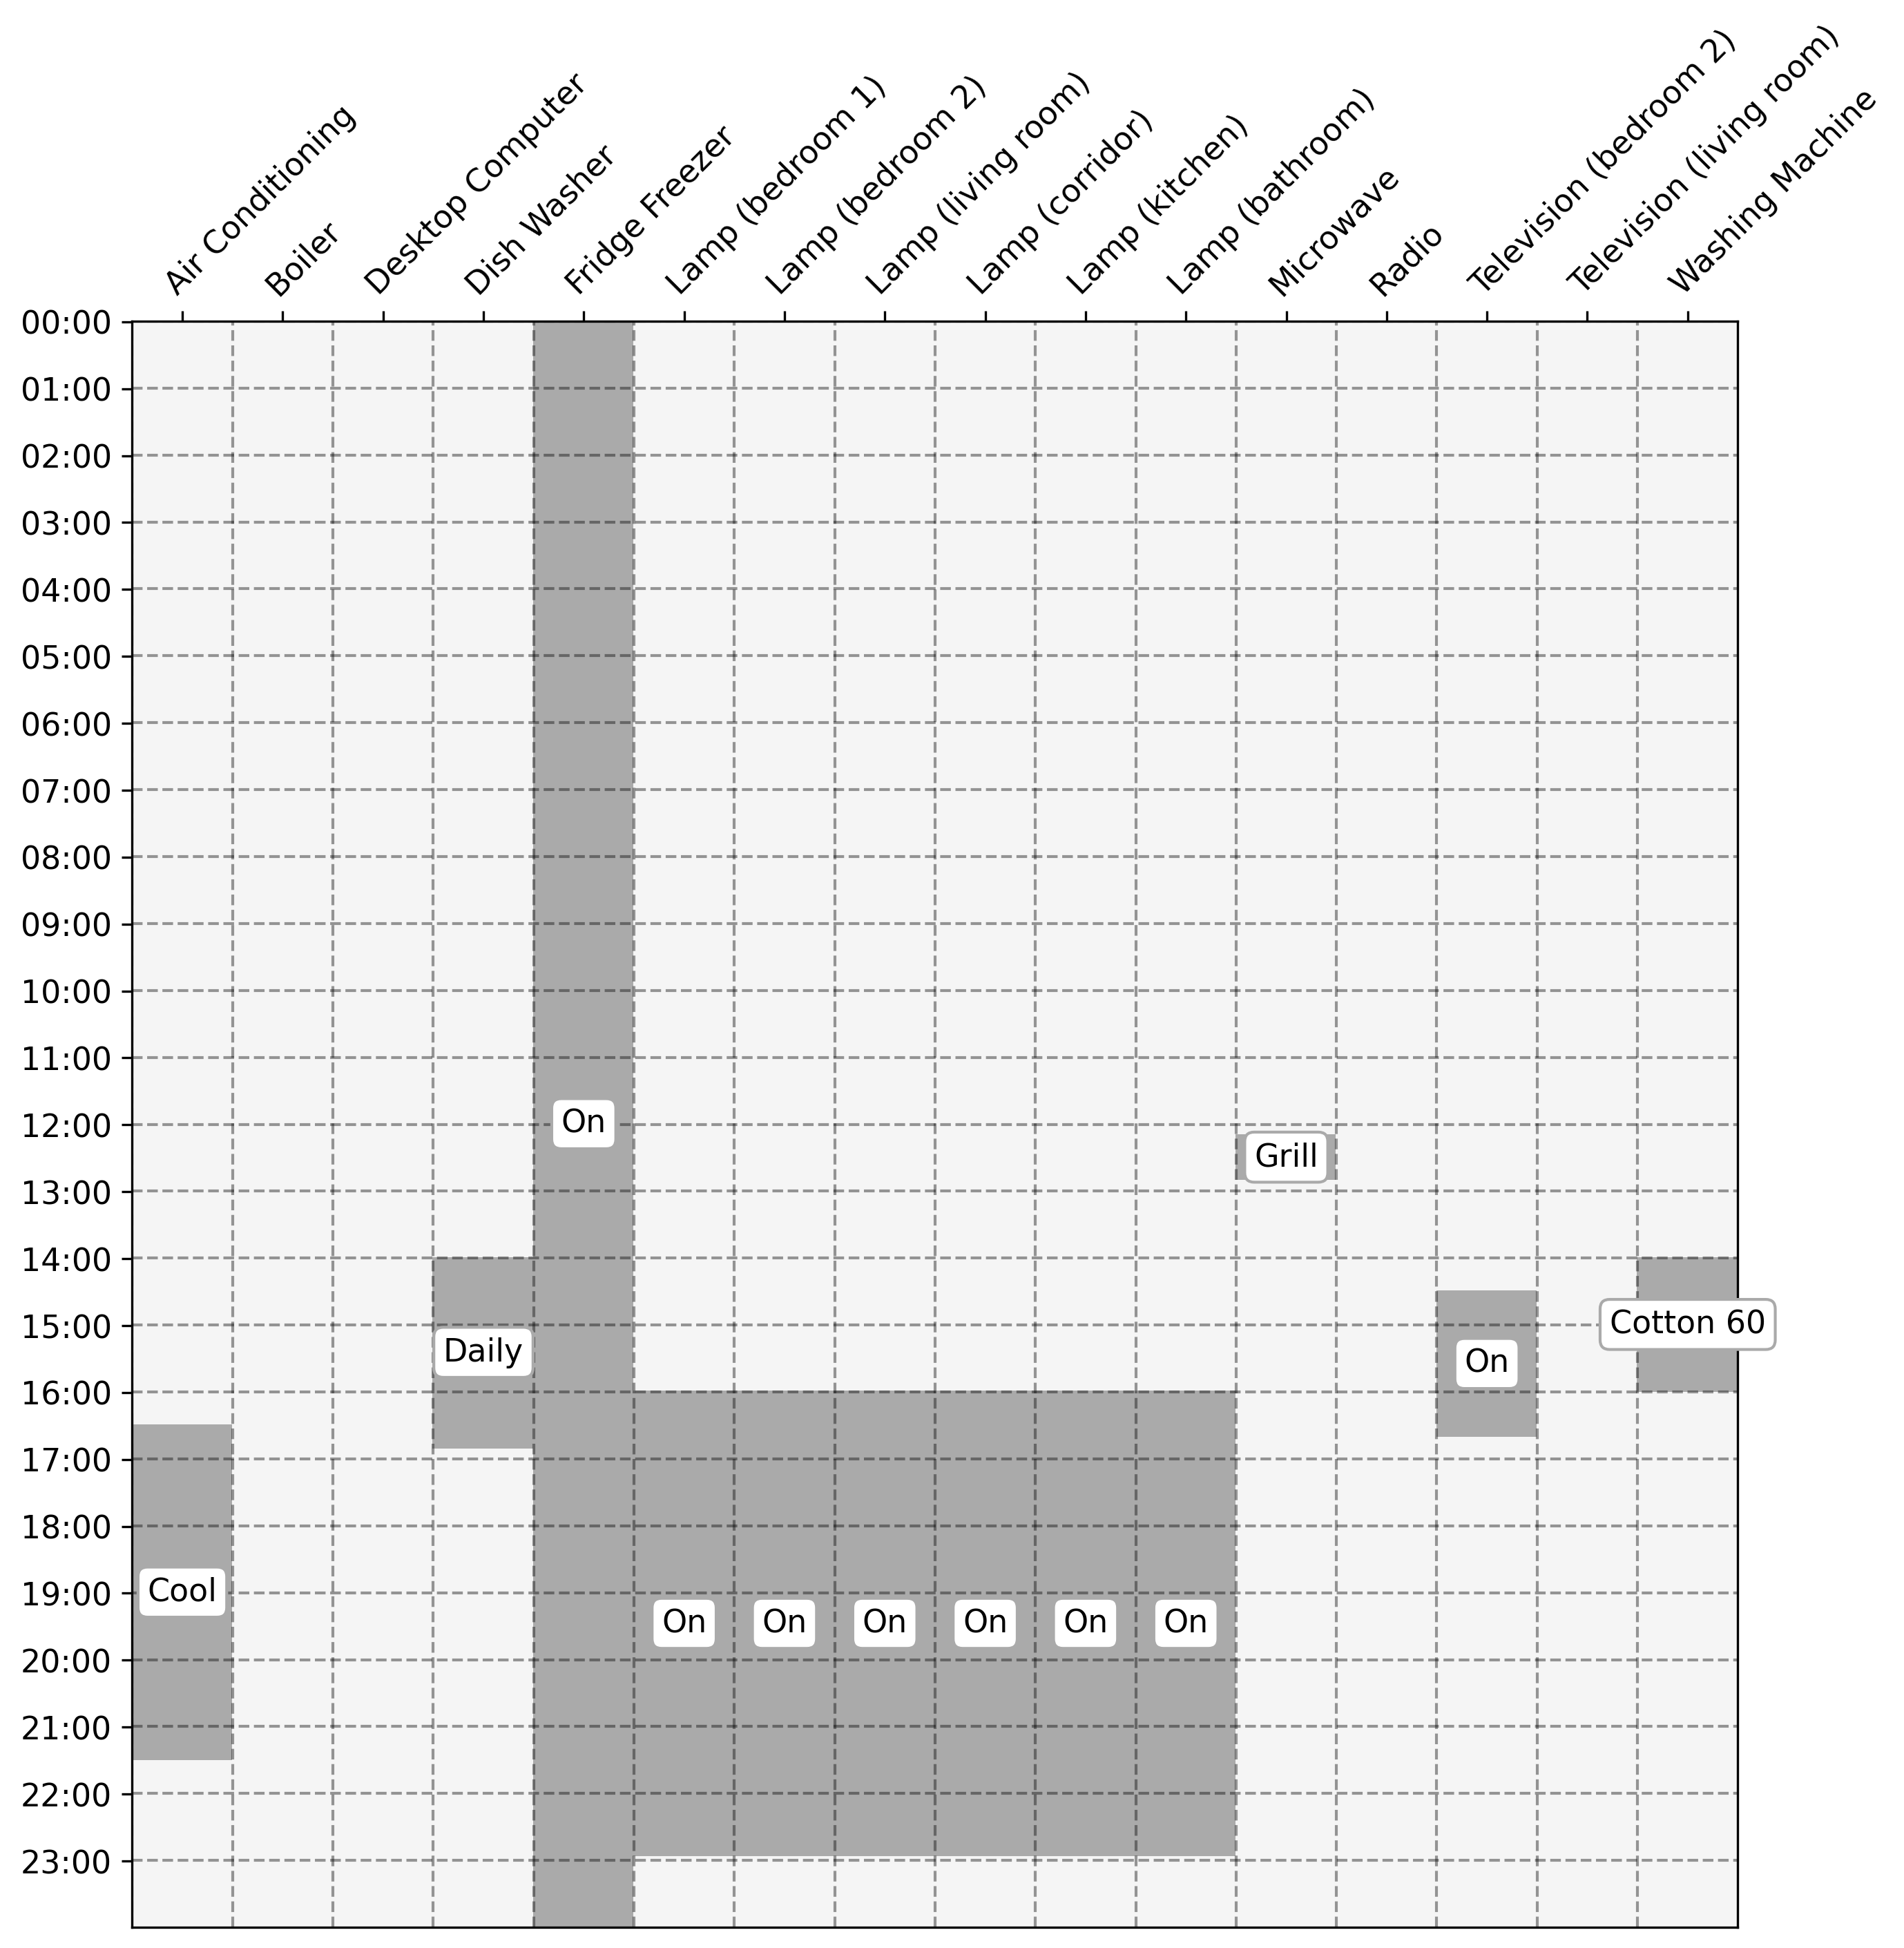
\includegraphics[width=0.9\textwidth]{images/real_matrix.png}
    \caption[Example of a state matrix]{Example of a state matrix. The matrix shows the operation modes of the appliances in the hypothetical home throughout the day, using a predefined set of routines}
    \label{fig:state_matrix}
\end{figure}

The matrix is implemented using the \texttt{ndarray} class provided by the NumPy library~\parencite{harrisArrayProgrammingNumPy2020}, which is a n-dimensional array of integers. As described in the Numpy N-Dimensional Array Reference\footnote{\url{https://numpy.org/doc/1.26/reference/arrays.ndarray.html}}, an instance of the \texttt{ndarray} class consists of a contiguous monodimensional memory segment, which combined with an indexing scheme allows to represent multidimensional arrays, mapping integers to the various elements that compose the memory block.

Each row of the matrix corresponds a minute of the day, and each column represents an appliance, by associating the appliance ID to the column index. For example, the first column of the matrix (index $0$) corresponds to the appliance with index 0. The value of each cell is the ID of the operation mode in which the appliance is set at that minute. Given that in a day there are $24 \times 60 = 1440$ minutes, and the hypothetical home has 15 appliances, the state map is a $1440 \times 15$ matrix. The type of the matrix is \textit{uint8}, which allows to store integers from 0 to 255, which is enough to store the IDs of the operation modes of the appliances. The total memory used by the state map is $1440 \times 15 \times 8 = 172800$ bits, which corresponds to roughly $21$ kilobytes.

Using the state matrix, calculating the consumption of an appliance at a given time of the day is straightforward. It is sufficient to index the matrix with the minute of the day and the appliance ID. The obtained value is the ID of the operation mode of the appliance at that time, and it can be used to get the energy consumption of the mode from the appliance's JSON file. To get the total energy consumption at a given time of the day, it is sufficient to sum the energy consumption of the single appliances at that time.

\section{Simulation of New Routines}\label{sec:simulation}

When simulating the addition of a new routine, it is possible that it causes a conflict with the existing routines. The \acrshort{dt} is capable of evaluating such conflicts and shows proper messages to the user. It is assumed that the existing routines are already consistent and conflict-free.

The \acrshort{dt} evaluates the potential conflicts and produces \textit{errors} or \textit{recommendations}, or both. An error occurs when a conflict creates an inconsistency among the routines, e.g. when two routines include actions that contradict each other, or that put the power draw over a maximum limit. Errors halt the simulation and prevent further evaluation. Recommendations are either warnings about minor conflicts that do not affect the consistency, or suggestions to improve the user experience or save energy. A recommendation does not interrupt the simulation and allows for further evaluation. This means that the digital twin can provide multiple recommendations for different conflicts, but at most one error is returned at a time.

The expected conflict scenario are the following:
\begin{enumerate}[label={\textit{S\arabic*.}}, leftmargin=3.5em]
    \item \textit{An appliance has conflicting operation modes in the same time interval}. This occurs when a simulated routine assigns an appliance a different operation mode than the one assigned by the existing routines in the same time interval. If the simulated routine assigns the same operation mode as the existing routines, there is no conflict. For instance, the AC is set to \textit{heat} from 8:00 to 12:00. A simulated routine that sets the AC to \textit{cold} from 10:00 to 11:00 causes a conflict. The digital twin rejects the simulated routine with an error that specifies the conflicting action and the existing routine and action. It also suggests deactivating the existing routine instead. This may be useful, for example, in weather conditions with sudden temperature changes, where the user may want to adjust the AC temporarily. If the simulated routine does not cause an inconsistency, e.g. it sets the AC to \textit{heat} from 11:00 to 13:00, then the digital twin accepts the simulated routine with a recommendation to modify the existing routine action to set \textit{heat} from 8:00 to 13:00.

    \item \textit{The power consumption exceeds a maximum limit at any time}. The digital twin rejects any routine that causes the power consumption to go beyond the maximum limit at any point. This limit could be the maximum power supply before cut off, e.g. $3kW$ in Italy. For example, if the microwave is in \textit{microwave mode}, the dishwasher is in \textit{intensive} mode, and the simulated routine sets the washing machine to \textit{cotton 60} mode at 14:00, the digital twin produces an error and advises a better start time for the washing machine.

    \item \textit{A better start time can be determined}. The digital twin tries to find a more economical start time for each action of the simulated routine, using pre-set electricity costs. This is important, for example, if the user has a variable electricity tariff, where it is less expensive to run appliances at night. If the electricity cost is constant throughout the day, this step can be ignored. The digital twin evaluates each action of the simulated routing sequentially, taking into account the best start time of the previous actions. For instance, if the best start time of action 1 of the simulated routine is 15:30, the digital twin should use that as a reference when evaluating action 2.

    \item \textit{An appliance is activated manually by the end user}. This scenario requires the digital twin to monitor the running state of appliances, in addition to the routines. Before executing any routine actions, the digital twin should check for conflicts with scenarios S1 and S2, using the current state of the appliances as well. If the scenarios produce an error, the conflicting actions should be prevented from running. Actions that are conflict-free can still be executed. Any recommendation produced can be displayed to the user to alert them and offer alternatives on what to do.
\end{enumerate}
The implementation of the digital twin developed for this thesis only covers conflicts S1-S4, while conflict S5 is left as a future development.

\begin{figure}
    \centering
    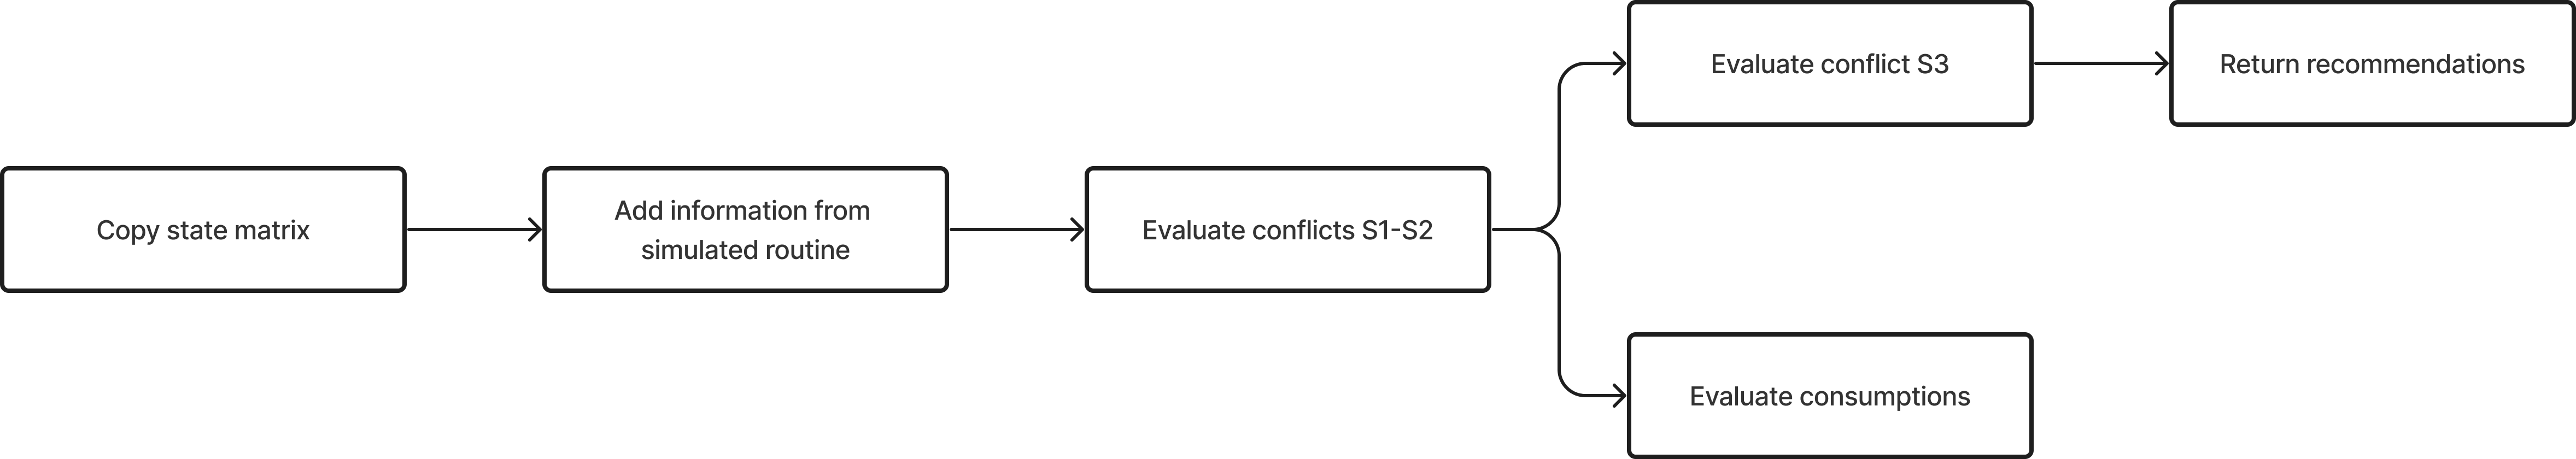
\includegraphics[width=\textwidth]{images/simulation_procedure.png}
    \caption{Simulation procedure}
    \label{fig:simulation_procedure}
\end{figure}

The complete procedure for simulating the addition of a new routine is shown in Figure~\ref{fig:simulation_procedure}. The procedure begins by creating a copy of the state matrix, using Numpys \texttt{copy} method. The new matrix is then updated to include the new appliance states from the simulated matrix. The procedure then evaluates the conflicts listed above, and stops when there is an error. An example of a simulated matrix obtained from adding a new routine to the matrix in Figure~\ref{fig:state_matrix} is shown in Figure~\ref{fig:simulated_consumption_matrix}. The \texttt{/simulate} endpoint of the \acrshort{api} returns the list of recommendations and errors, if any. The other simulation endpoints of the \acrshort{api} instead do not return any recommendation, but instead compute consumption values on the new state matrix. Any error is returned anyway.

\begin{figure}
    \centering
    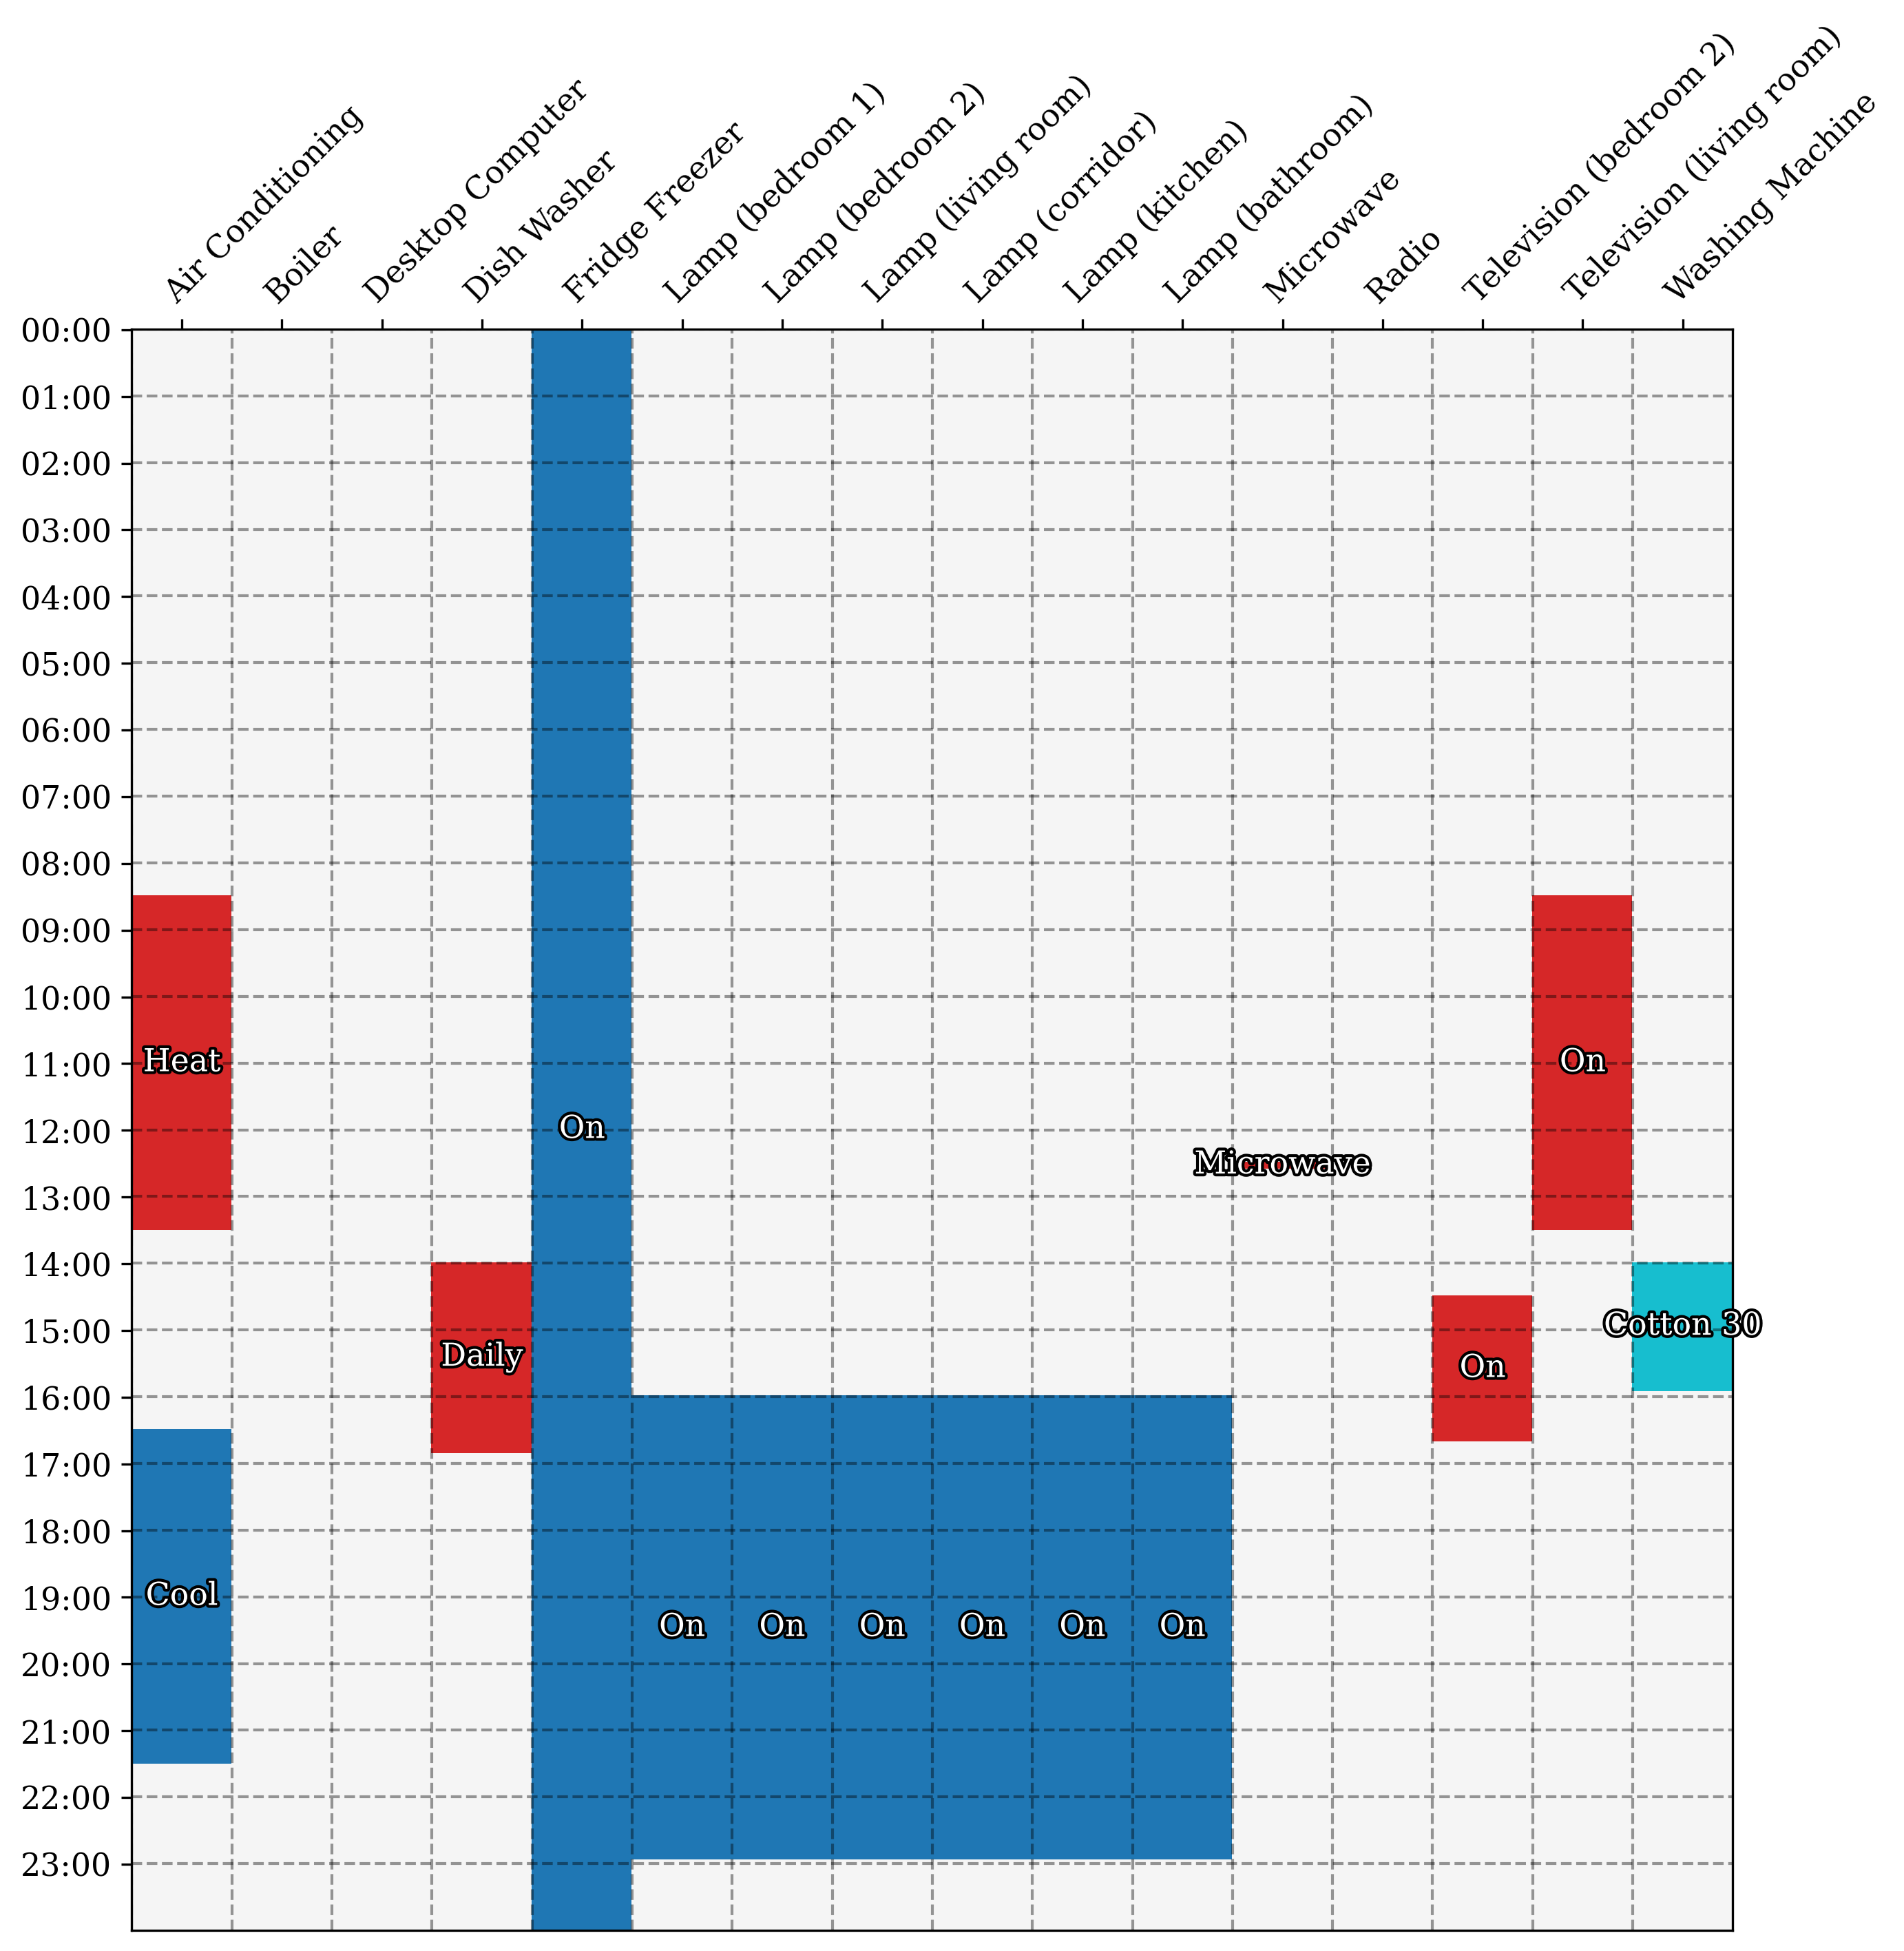
\includegraphics[width=0.9\textwidth]{images/simulated_matrix.png}
    \caption{Simulated matrix}
    \label{fig:simulated_consumption_matrix}
\end{figure}

In order to find the best start time according to S3, the \acrshort{dt} uses a brute force approach, by evaluating the energy cost of starting the simulated routine at each minute of the day, and selecting the one with the lowest cost. The energy cost of a routine is calculated by summing the cost of starting each of the actions at the selected time, using the energy rates provided in the configuration file. This operation is repeated 1440 times, once for each minute of the day. The \acrshort{dt} then returns the best start time, along with the monetary savings of starting the routine at that time. The monetary savings are calculated by comparing the cost of starting the routine at the best start time with the cost of starting the routine at the time specified in the routine. 

\section{Frontend}

The frontend application is meant to showcase the functionalities of the \acrshort{dt}, and it is not meant to be a fully functional interface for end users. To reflect this, it is launched separately from the \acrshort{rest} \acrshort{api}. It shows, among other things, the energy consumption of appliances during the day, simulates the addition of new routines evaluating eventual conflicts with the existing routines. The frontend application is also capable of showing the list of appliances and routines in the home, and allows the user to add new routines.

The frontend is developed using the React\footnote{\url{https://react.dev/}} framework, which is a JavaScript library for building user interfaces. React is chosen for its simplicity and performance, as it is based on a component-based architecture, which allows to build complex user interfaces by composing small and isolated pieces of code. The styling of the frontend is done using the Tailwind CSS \footnote{\url{https://tailwindcss.com/}} library, which is a utility-first CSS framework that allows to build custom designs without having to write custom CSS. The FlowBite\footnote{\url{https://flowbite.com/}} library is used to provide a set of pre-built TailwindCSS components, which also support dark mode.

The application is also designed to be \textit{responsive}, meaning that it adapts to different screen sizes, and is usable on both desktop and mobile devices. The application is also capable of handling multiple requests concurrently, and is designed to be scalable and easy to maintain~\parencite{marcotteResponsiveWebDesign2010}. It should be noted however that some elements of the page, such as tables, are not easily readable on mobile devices.

\subsection{Header Section}

The header in Figure~\ref{fig:frontend_header} is shown on top of the application. It contains the title and logo of the application, taken from Material Icons\footnote{\url{https://fonts.google.com/icons}}. On the right side of the header, there are two buttons: one to toggle the app to and from the dark mode, and the other to open the \acrshort{api} documentation.

\begin{figure}
    \centering
    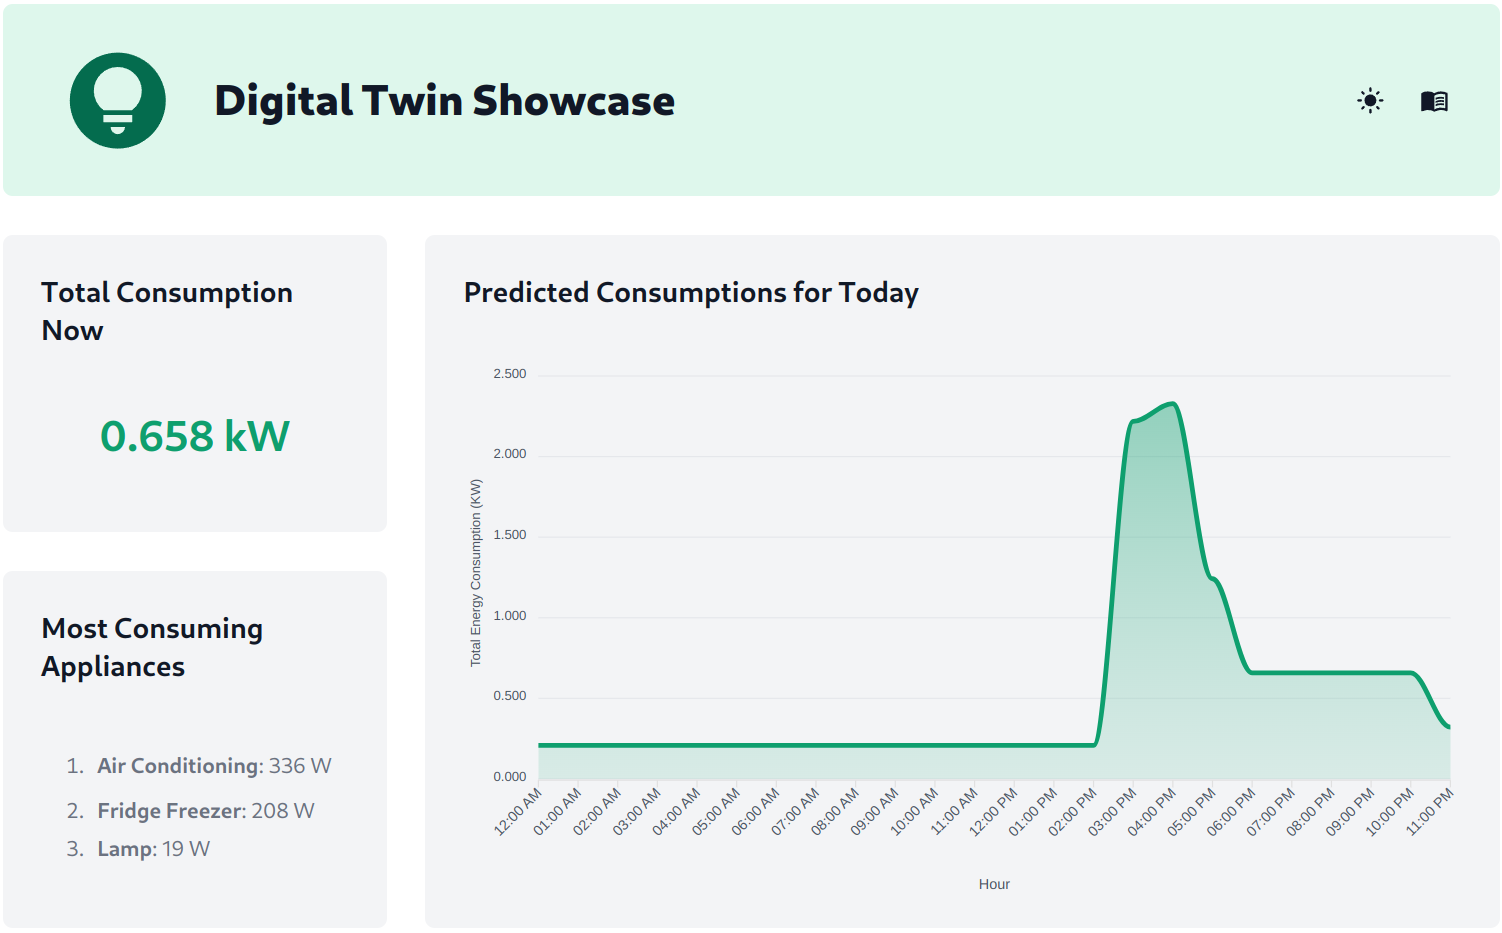
\includegraphics[width=0.9\textwidth]{images/frontend/header.png}
    \caption{Header of the frontend application}
    \label{fig:frontend_header}
\end{figure}

\subsection{Statistics Section}

The statistics section shows various informations about the home, including the total energy consumption of all appliances at the current time, the three most consuming appliances at the current time and their power consumption, and a chart showing the predicted total energy consumption of all appliances during the day. The chart is is implemented using the ApexCharts\footnote{\url{https://apexcharts.com/}} library, and includes funcionalities such as zooming and panning, and tooltips to show more information about data points.

\begin{figure}
    \centering
    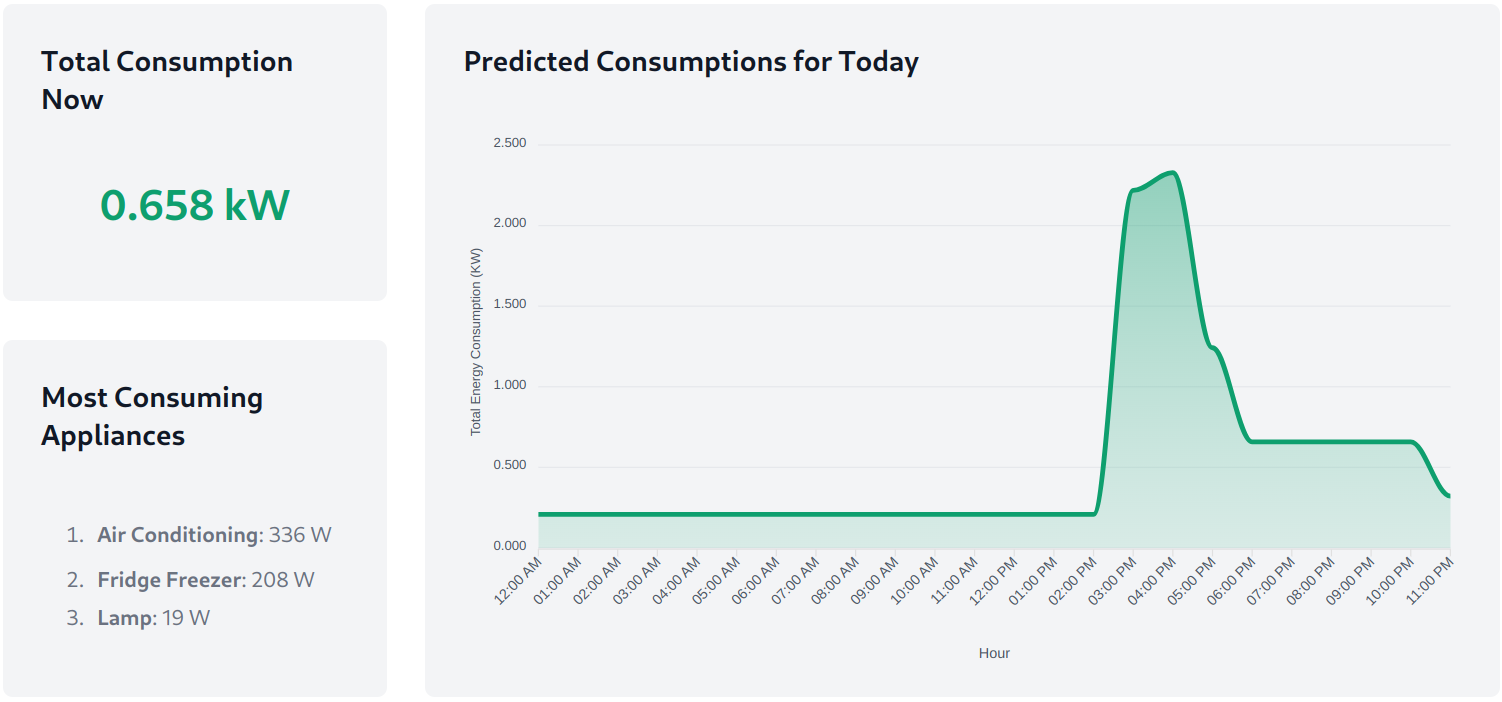
\includegraphics[width=0.9\textwidth]{images/frontend/statistics.png}
    \caption{Statistics section of the frontend application}
    \label{fig:frontend_statistics}
\end{figure}

\subsection{Simulate Section}

The simulate section of the application, shown in Figure~\ref{fig:frontend_simulate}, allows the user to simulate the addition of a new routine, evaluating eventual conflicts with the existing routines. The user can select one of three predefined routines through a tab interface, meant to showcase the different outputs of the simulation procedure.

\begin{figure}
    \centering
    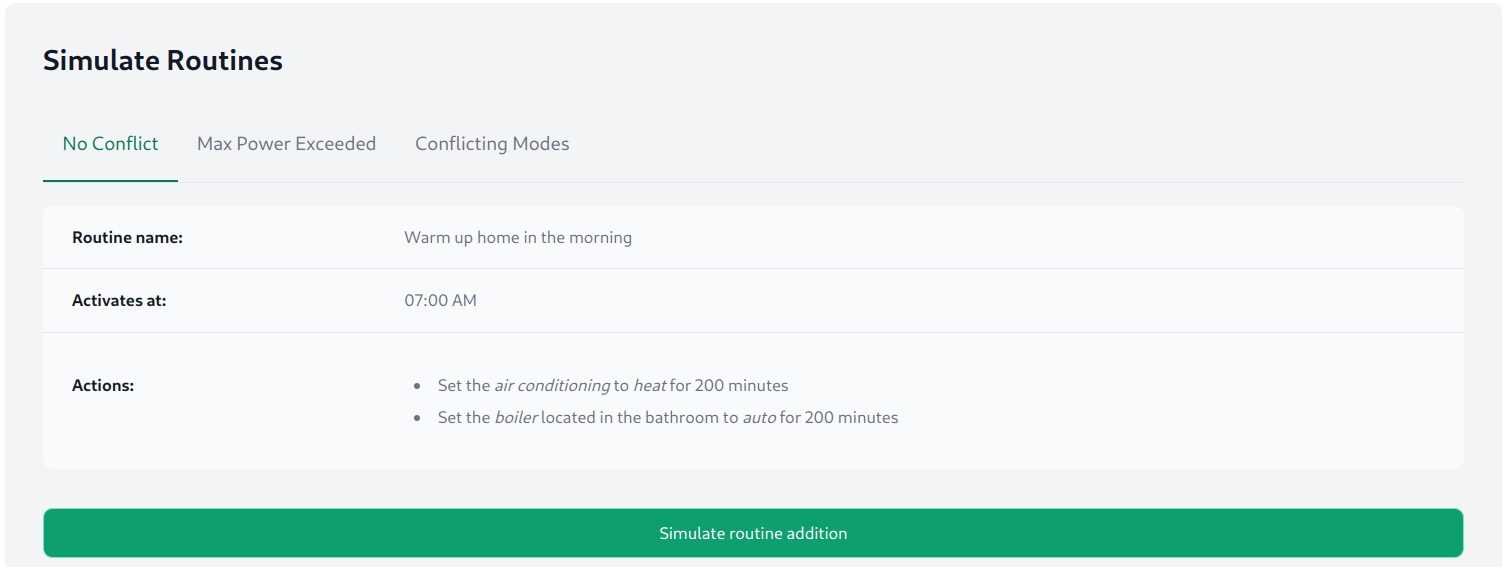
\includegraphics[width=0.9\textwidth]{images/frontend/simulate.png}
    \caption{Simulate section of the frontend application}
    \label{fig:frontend_simulate}
\end{figure}

The default "No Conflict" tab shows the "Warm up home in the morning" routine which starts the air conditioning and boiler at 7:00 AM. Pressing the "Simulate routine addition" button sends a \texttt{POST} request to the \texttt{/simulate} endpoint of the \acrshort{api}. The result of the simulation is shown in Figure~\ref{fig:frontend_no_conflict_result}, which shows that the routine is accepted. A graph comparing the consumptions with and without the simulated routines is shown, which is populated using the data from the \texttt{/simulate/consumption/total} endpoint of the \acrshort{api}. A recommendation with a suggestion to change the start time of the routine is also shown. The savings are projected over a time period of 30 days, in order to show a more significant monetary value.

\begin{figure}
    \centering
    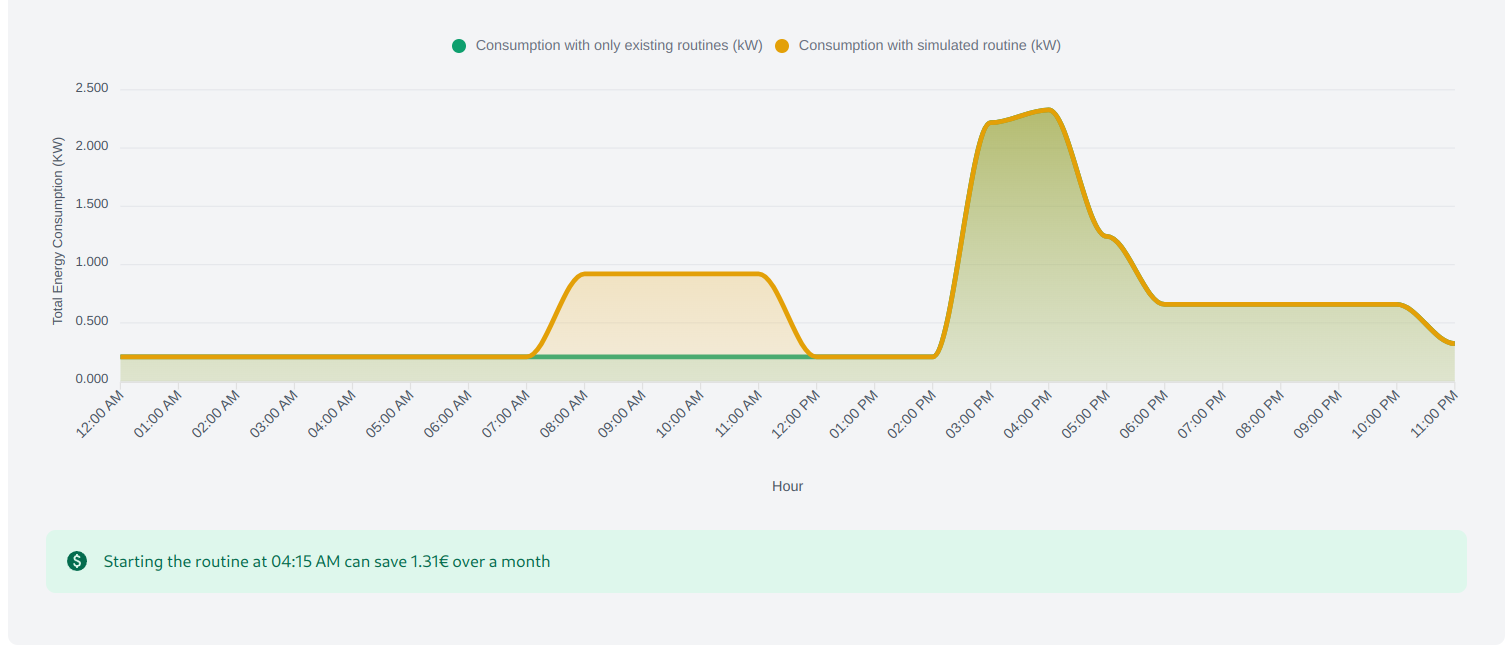
\includegraphics[width=0.9\textwidth]{images/frontend/no_conflict_result.png}
    \caption{Results of simulating the "Warm up home in the morning" routine}
    \label{fig:frontend_no_conflict_result}
\end{figure}

The routine "Party time" in Figure~\ref{fig:frontend_max_power_exceeded} is designed so that the power consumption exceeds the maximum limit of 3kW. It starts the air conditioning, the dishwasher, the washing machine, and the microwave at 10:00 AM. The results of the simulation are shown in Figure~\ref{fig:frontend_max_power_exceeded_result}. The routine produces an error, caused by conflict S2, and a recommendation to disable the simulated routine or an existing routine that causes high energy draw. No recommendation with a more appropriate start time is shown, because starting the simulated routine at any time of the day causes the power consumption to exceed the maximum limit.

\begin{figure}
    \centering
    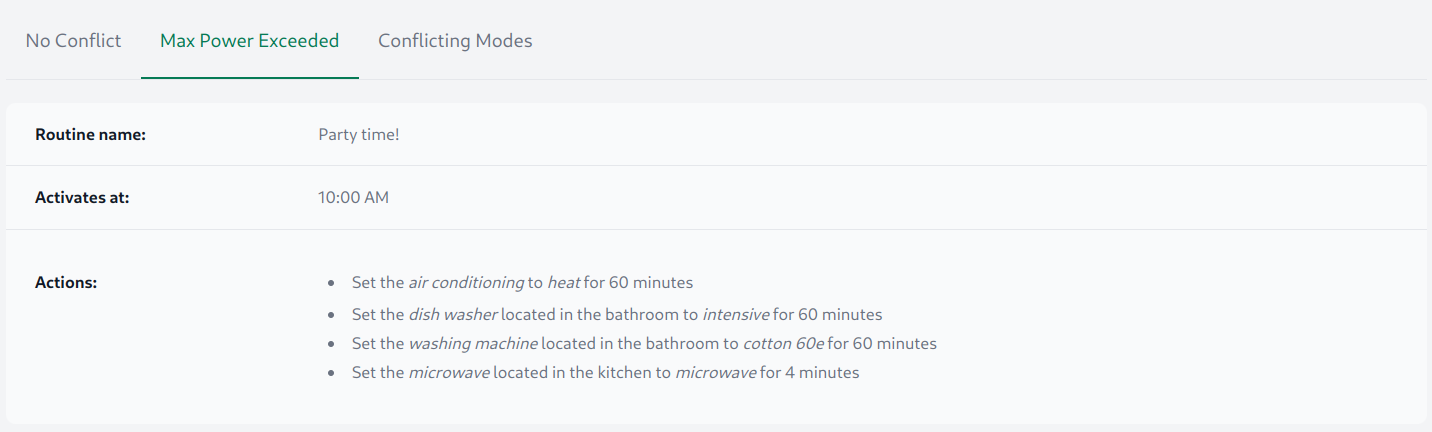
\includegraphics[width=0.9\textwidth]{images/frontend/max_power_exceeded.png}
    \caption{Details of the "Party time" routine, which causes the power consumption to exceed the maximum limit}
    \label{fig:frontend_max_power_exceeded}
\end{figure}

\begin{figure}
    \centering
    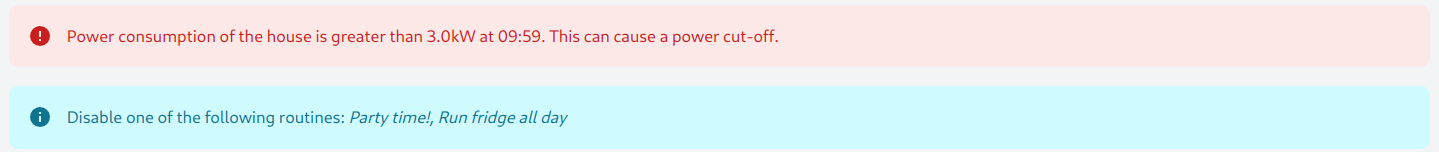
\includegraphics[width=0.9\textwidth]{images/frontend/max_power_exceeded_result.png}
    \caption{Result of simulating the "Party time" routine}
    \label{fig:frontend_max_power_exceeded_result}
\end{figure}

The routine "Heavy duty wash" in Figure~\ref{fig:frontend_conflicting_modes} is designed to cause a conflict with an existing routine. It starts the washing machine in \textit{cotton 90} mode at 14:00. However, at the same time, another routine already sets the washing machine to the "Cotton 30" mode. The results of the simulation are shown in Figure~\ref{fig:frontend_conflicting_modes_result}. The routine produces an error, caused by conflict S1, two recommendations to disable each of the conflicting routines (shown in the same message), and a recommendation to change the start time of the routine, again with the monetary savings of doing so.

\begin{figure}
    \centering
    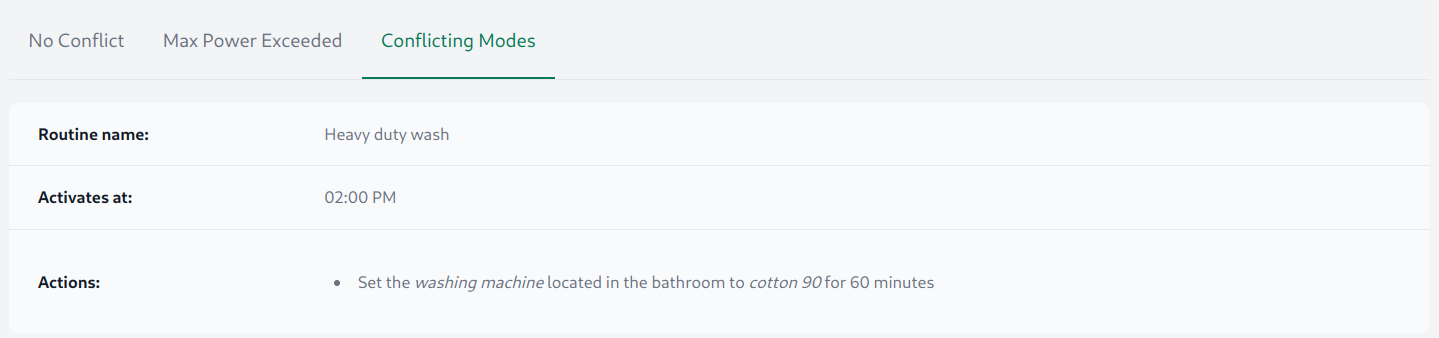
\includegraphics[width=0.9\textwidth]{images/frontend/conflicting_modes.png}
    \caption{Details of the "Heavy duty wash" routine, which causes a conflict with an existing routine}
    \label{fig:frontend_conflicting_modes}
\end{figure}

\begin{figure}
    \centering
    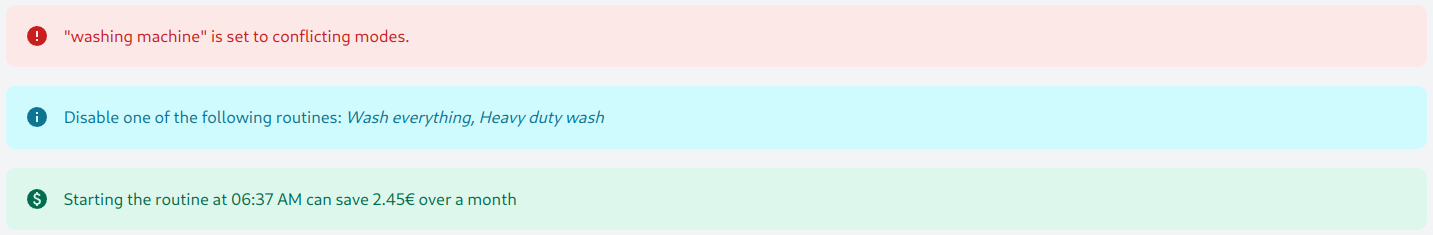
\includegraphics[width=0.9\textwidth]{images/frontend/conflicting_modes_result.png}
    \caption{Result of simulating the "Heavy duty wash" routine}
    \label{fig:frontend_conflicting_modes_result}
\end{figure}

\subsection{Appliances Section}

The appliances section of the application is shown in Figure~\ref{fig:frontend_appliances}. The section shows a table with the list of appliances in the home. The table includes the device, manufacturer, model, location of the appliances in the home, and the name of the supported operation modes. The table also automatically adds an appropriate icon for each appliance, taken from Material Icons.

\begin{figure}
    \centering
    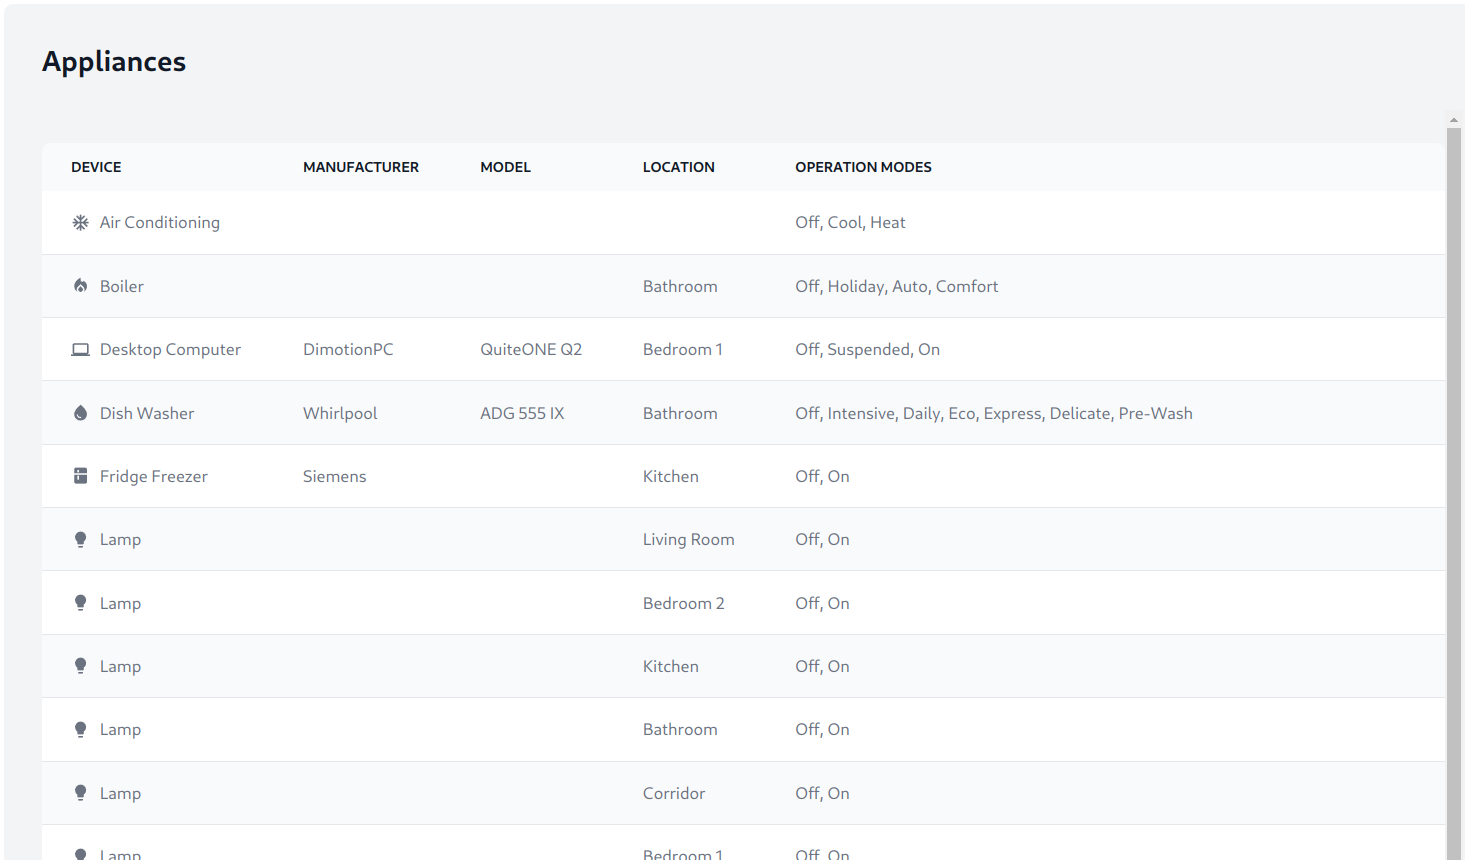
\includegraphics[width=0.9\textwidth]{images/frontend/appliances.png}
    \caption{Simulate Section of the Frontend Application}
    \label{fig:frontend_appliances}
\end{figure}

\subsection{Routines Section}

Similarly to the appliances section, the routines section of the application is shown in Figure~\ref{fig:frontend_routines}. The section shows a table with the list of routines in the home. The table includes the name, time of activation of the routines, whether the routine is enabled or not, and the list of actions of the routines.

\begin{figure}
    \centering
    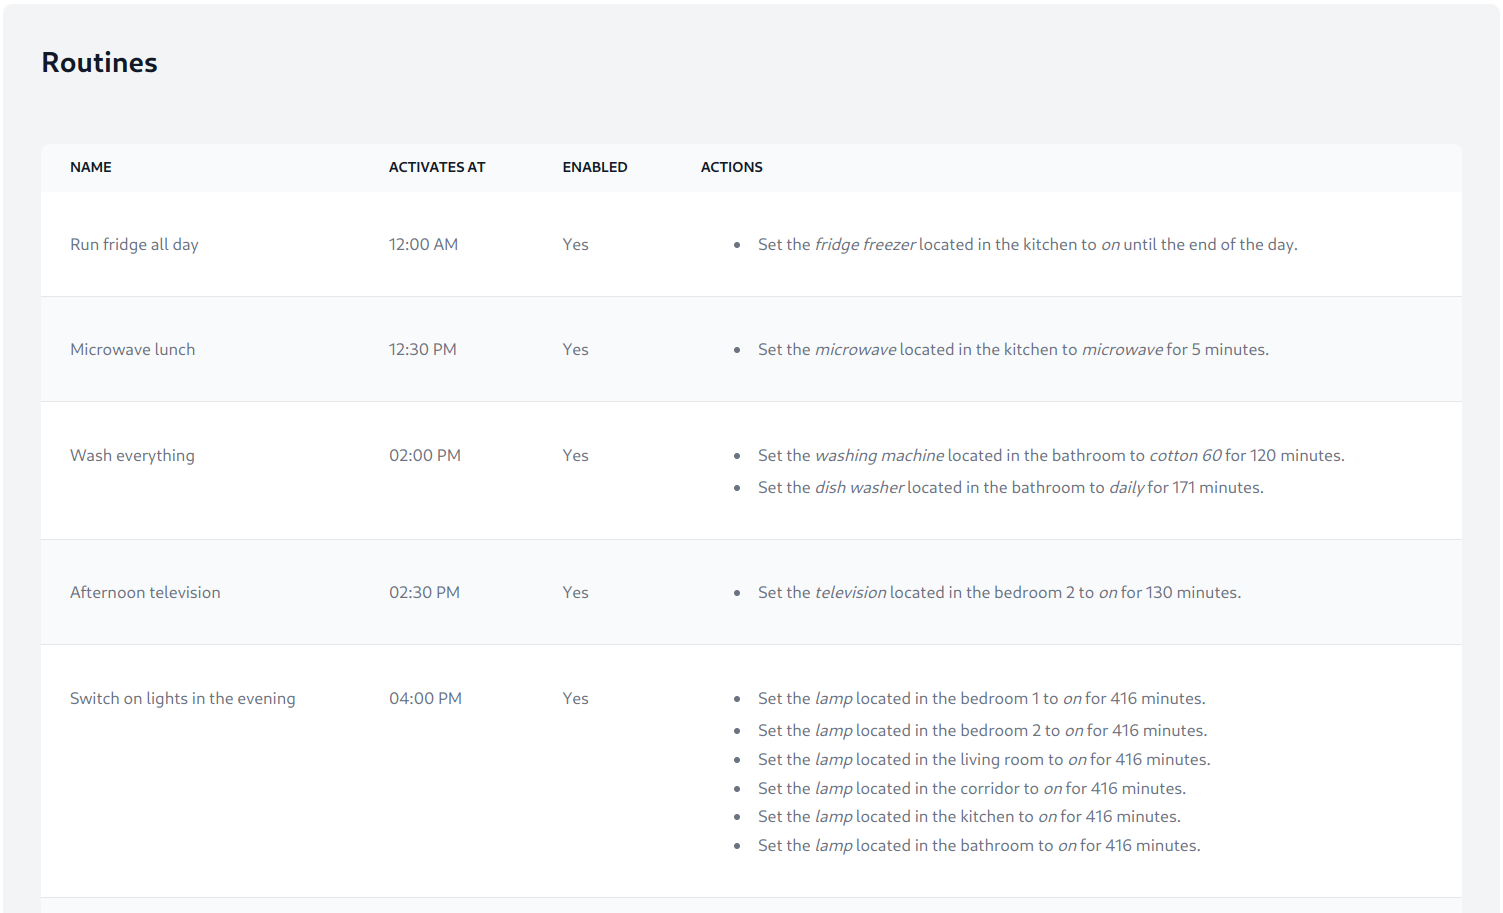
\includegraphics[width=0.9\textwidth]{images/frontend/routines.png}
    \caption{Showcase Frontend Application}
    \label{fig:frontend_routines}
\end{figure}